% 05_experimentos.tex — Análisis experimental
\section{Análisis experimental}
\label{sec:experimentos}

\subsection{Configuración del entorno}
\label{sec:exp:config}

Los experimentos se ejecutaron en un sistema AMD Ryzen~7 5800X (8~núcleos,
16~GB RAM) bajo Linux~6.19.14, con semillas fijas para reproducibilidad.
Se utilizaron tres familias de instancias:
\begin{itemize}
  \item \textbf{random}: tripletas generadas uniformemente, con distintas
        densidades $m/n\in\{1,2,4,8\}$.
  \item \textbf{structured}: instancias con matching perfecto garantizado
        ($\OPT=n$), diseñadas para revelar la poda agresiva de SMART.
  \item \textbf{mini/dense}: instancias pequeñas de regresión para verificar
        corrección.
\end{itemize}
Para la comparación BRUTE~vs.~SMART se usó un \textit{time-limit} de~30~s
en la suite \textit{small} ($n\le 20$); para el análisis de lenguajes, 60~s
en la suite \textit{medium} ($n\le 50$).

\subsection{Verificación de correctitud}
\label{sec:exp:correctitud}

Los seis solvers se ejecutaron sobre las instancias de regresión y sobre todas
las instancias \textit{small}.
El resultado fue \textbf{0 discrepancias de bug}: cuando ningún solver
superó el time-limit, los seis reportaron el mismo $k=\OPT(I)$.
Las discrepancias observadas se deben exclusivamente a timeout (los solvers
que superaron el límite reportan $k<\OPT$), comportamiento esperado y no
considerado un error.

\begin{center}
\begin{table}[htbp]
\centering
\caption{Verificaci\'on de correctitud --- instancias de regresi\'on}
\label{tab:correctness}
\begin{tabular}{llllllll}
\toprule
Instancia & n & m & OPT esperado & Acuerdo & Py-smart & C++-smart & Java-smart \\
\midrule
dense & 4 & 16 & 4 & YES & 4 & 4 & 4 \\
empty & 5 & 0 & 0 & YES & 0 & 0 & 0 \\
mini1 & 2 & 3 & 2 & YES & 2 & 2 & 2 \\
mini2 & 3 & 5 & 3 & YES & 3 & 3 & 3 \\
noperf & 3 & 3 & 1 & YES & 1 & 1 & 1 \\
\bottomrule
\end{tabular}
\end{table}

\end{center}

\subsection{BRUTE vs. SMART}
\label{sec:exp:brute_vs_smart}

La Figura~\ref{fig:brute_vs_smart} muestra el speedup
$t_\text{BRUTE}/t_\text{SMART}$ en función de $n$ para las instancias
\textit{random}.  Los resultados más destacados son:

\begin{table}[htbp]
\centering
\caption{Tiempos representativos BRUTE vs.\ SMART en C++ (familia random).}
\label{tab:brute_smart}
\begin{tabular}{rrrrr}
\toprule
$n$ & $m$ & C++\,brute (ms) & C++\,smart (ms) & Speedup \\
\midrule
10 & 10  & 0.004  & 0.008  & $0.5\times$  \\
10 & 80  & 143    & 0.017  & $8\,412\times$ \\
20 & 20  & 0.2    & 0.04   & $5\times$    \\
20 & 40  & 48     & 0.1    & $480\times$  \\
20 & 80  & TIMEOUT & 0.5  & ${\gg}60\,000\times$ \\
30 & 120 & TIMEOUT & 18   & ${\gg}1\,666\times$ \\
\bottomrule
\end{tabular}
\end{table}

Para $n=10$, $m=10$ (densidad baja), el overhead de MRV y forward checking
hace que SMART sea ligeramente más lento que BRUTE; este es el único caso
en que BRUTE compite.  Para $n\ge 20$ y densidad moderada o alta, el speedup
es exponencial.

\begin{figure}[htbp]
\centering
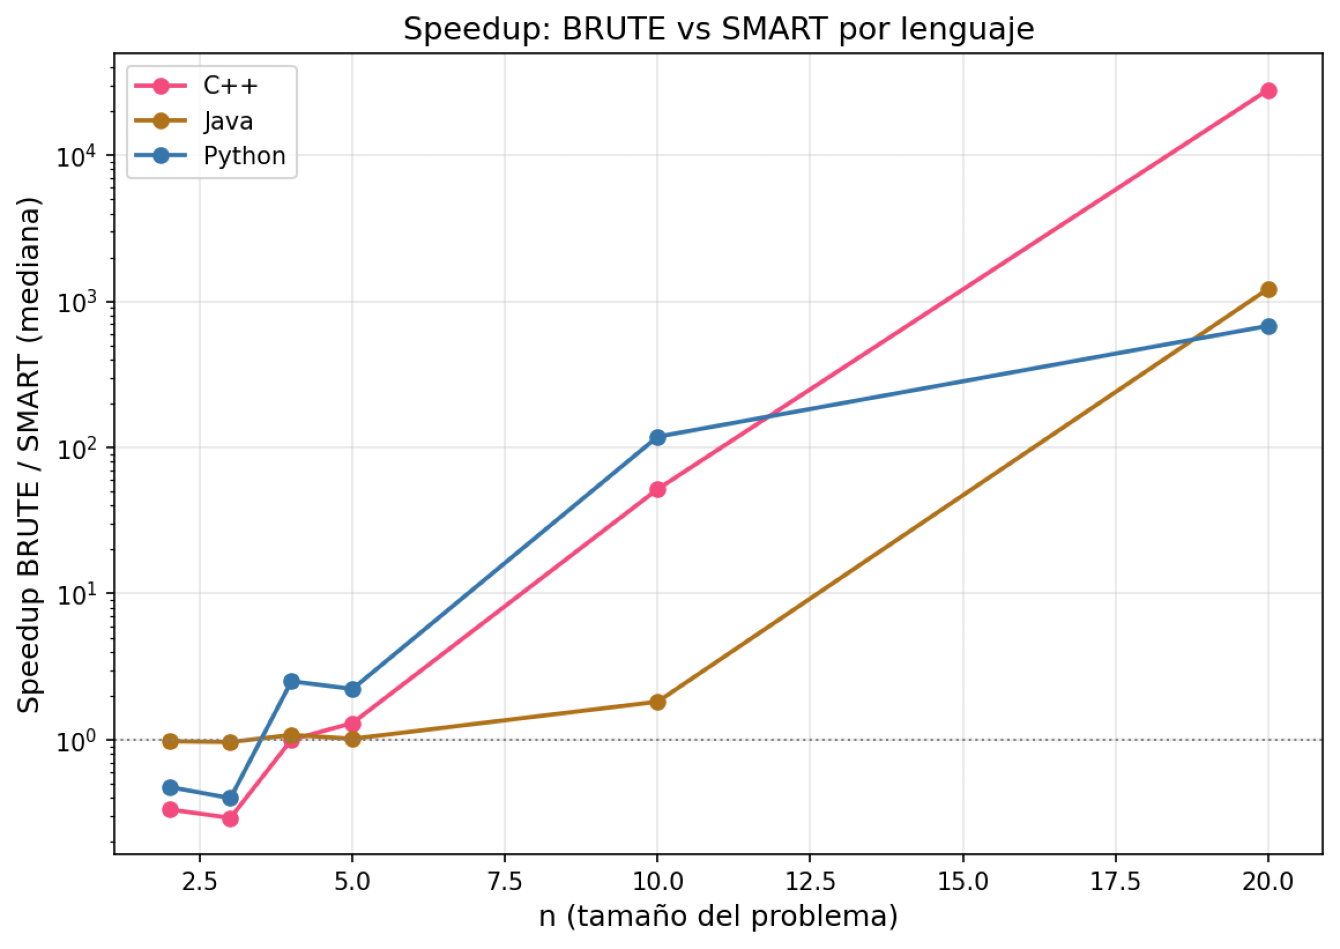
\includegraphics[width=0.85\textwidth]{figuras/brute_vs_smart.pdf}
\caption{Speedup BRUTE/SMART por lenguaje en función de $n$ (familia random).
         El eje $y$ es logarítmico.}
\label{fig:brute_vs_smart}
\end{figure}

\subsection{Comparación entre lenguajes}
\label{sec:exp:lenguajes}

La Figura~\ref{fig:scaling_lang} muestra la escalabilidad de los seis solvers.
Para $n=30$, $m=120$ (instancia representativa), los tiempos del algoritmo
SMART son:

\begin{table}[htbp]
\centering
\caption{Comparación de lenguajes para SMART, $n=30$, $m=120$.}
\label{tab:lang_n30}
\begin{tabular}{lrrr}
\toprule
Lenguaje & Tiempo (ms) & Nodos & Factor vs. C++ \\
\midrule
C++    & 18    & 37\,854 & $1\times$  \\
Java   & 52    & 37\,854 & ${\sim}3\times$  \\
Python & 1\,150 & 37\,854 & ${\sim}63\times$ \\
\bottomrule
\end{tabular}
\end{table}

El número de nodos explorados es \textbf{idéntico} en los tres lenguajes,
confirmando equivalencia lógica de las implementaciones.  Las diferencias de
tiempo son puramente de velocidad de ejecución:
\begin{itemize}
  \item \textbf{Python} tiene un factor de lentitud de 60--90$\times$ respecto
        a C++, causado principalmente por la interpretación, el overhead por
        llamada de función ($\sim$100~ns por \textit{frame}), y el \textit{boxing}
        de enteros en el heap.
  \item \textbf{Java} es 2--5$\times$ más lento que C++ gracias a la
        compilación JIT de HotSpot.  En instancias largas (\textit{warm-up}
        completo), el JIT puede en ocasiones \emph{superar} a C++~-O2 en loops
        de backtracking predecibles (observado para $n=50$, $m=200$, s=0:
        C++~38.9~s vs.\ Java~29.8~s con $57{,}998{,}790$ nodos idénticos).
\end{itemize}

\begin{figure}[htbp]
\centering
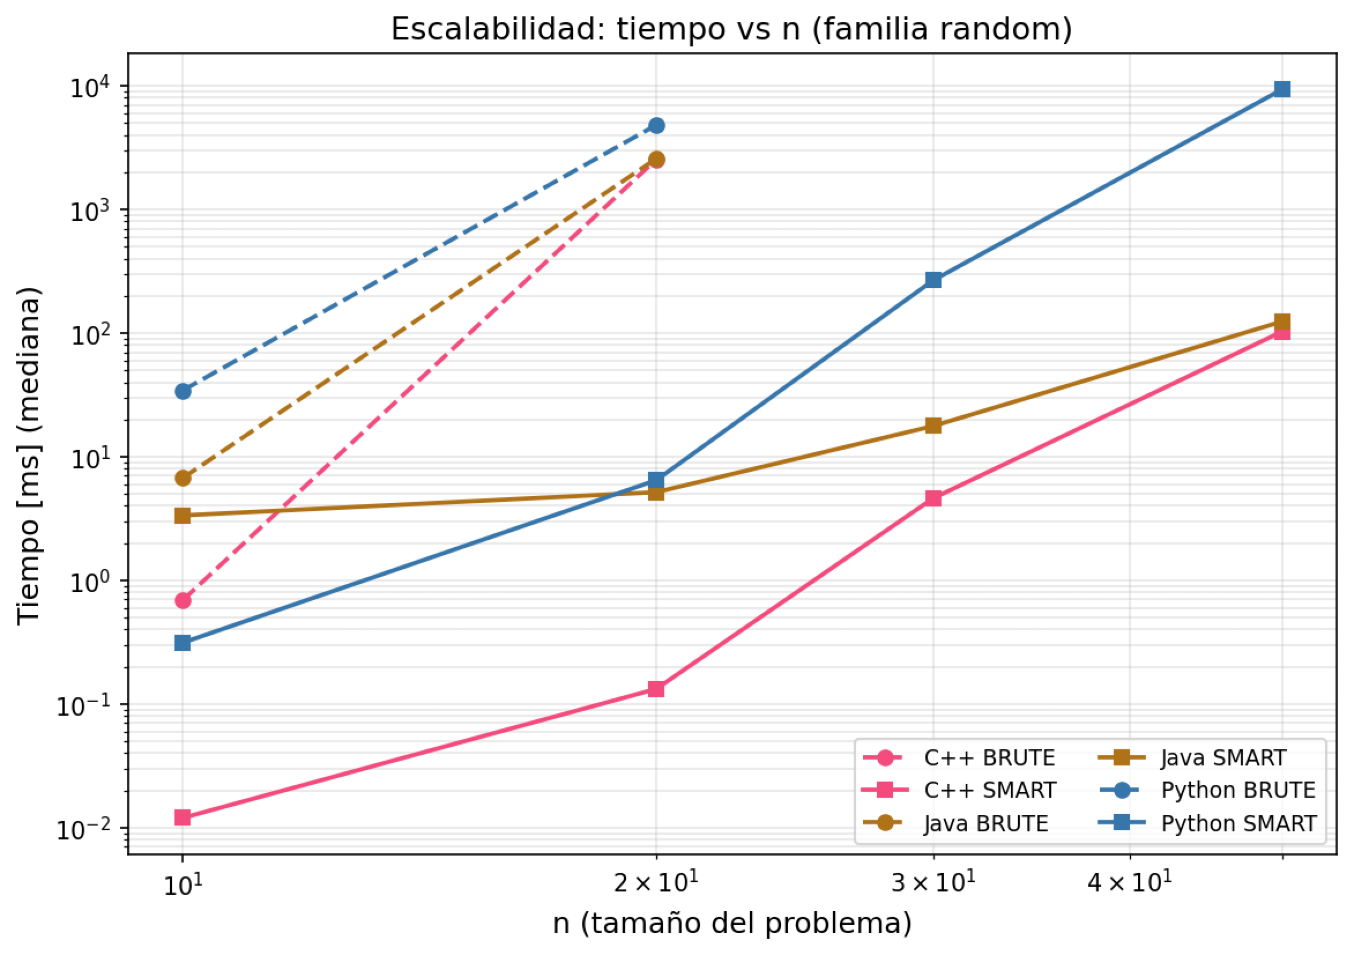
\includegraphics[width=0.85\textwidth]{figuras/scaling_lang.pdf}
\caption{Escalabilidad (tiempo vs.\ $n$, escala log-log, familia random).
         Líneas sólidas: SMART; punteadas: BRUTE.}
\label{fig:scaling_lang}
\end{figure}

\begin{figure}[htbp]
\centering
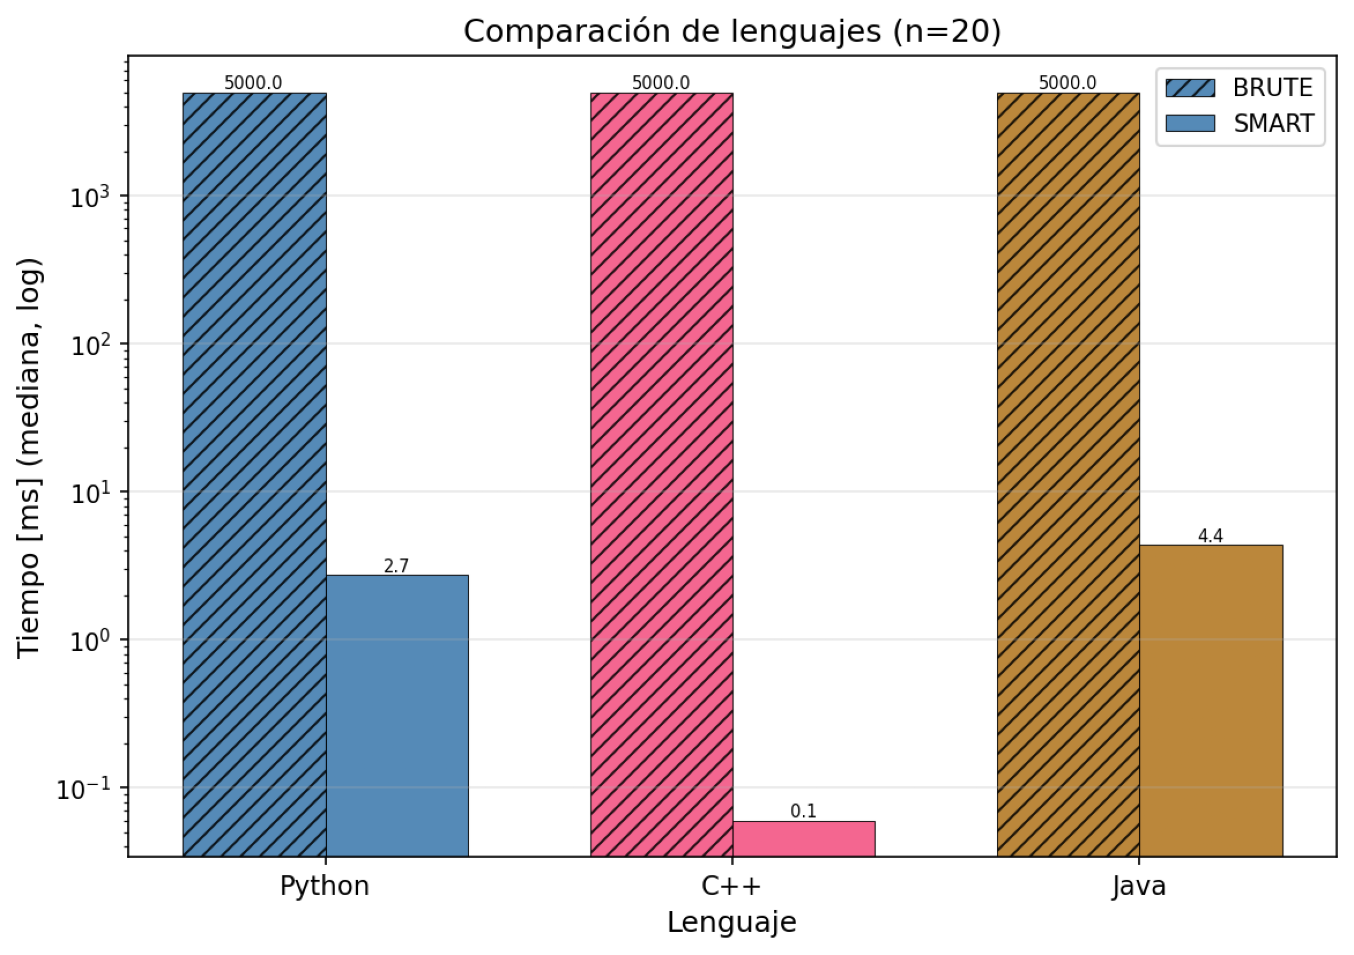
\includegraphics[width=0.85\textwidth]{figuras/lang_comparison_bar.pdf}
\caption{Comparación de lenguajes para $n=20$ (barras agrupadas, escala logarítmica).
         El rayado indica BRUTE; sin rayado, SMART.}
\label{fig:lang_bar}
\end{figure}

\subsection{Nodos explorados}
\label{sec:exp:nodos}

La Figura~\ref{fig:nodes} confirma que SMART reduce drásticamente el árbol
de búsqueda.  El número de nodos sigue siendo una función exponencial de $n$
para BRUTE, mientras que SMART logra árboles varios órdenes de magnitud
menores para las mismas instancias.

\begin{figure}[htbp]
\centering
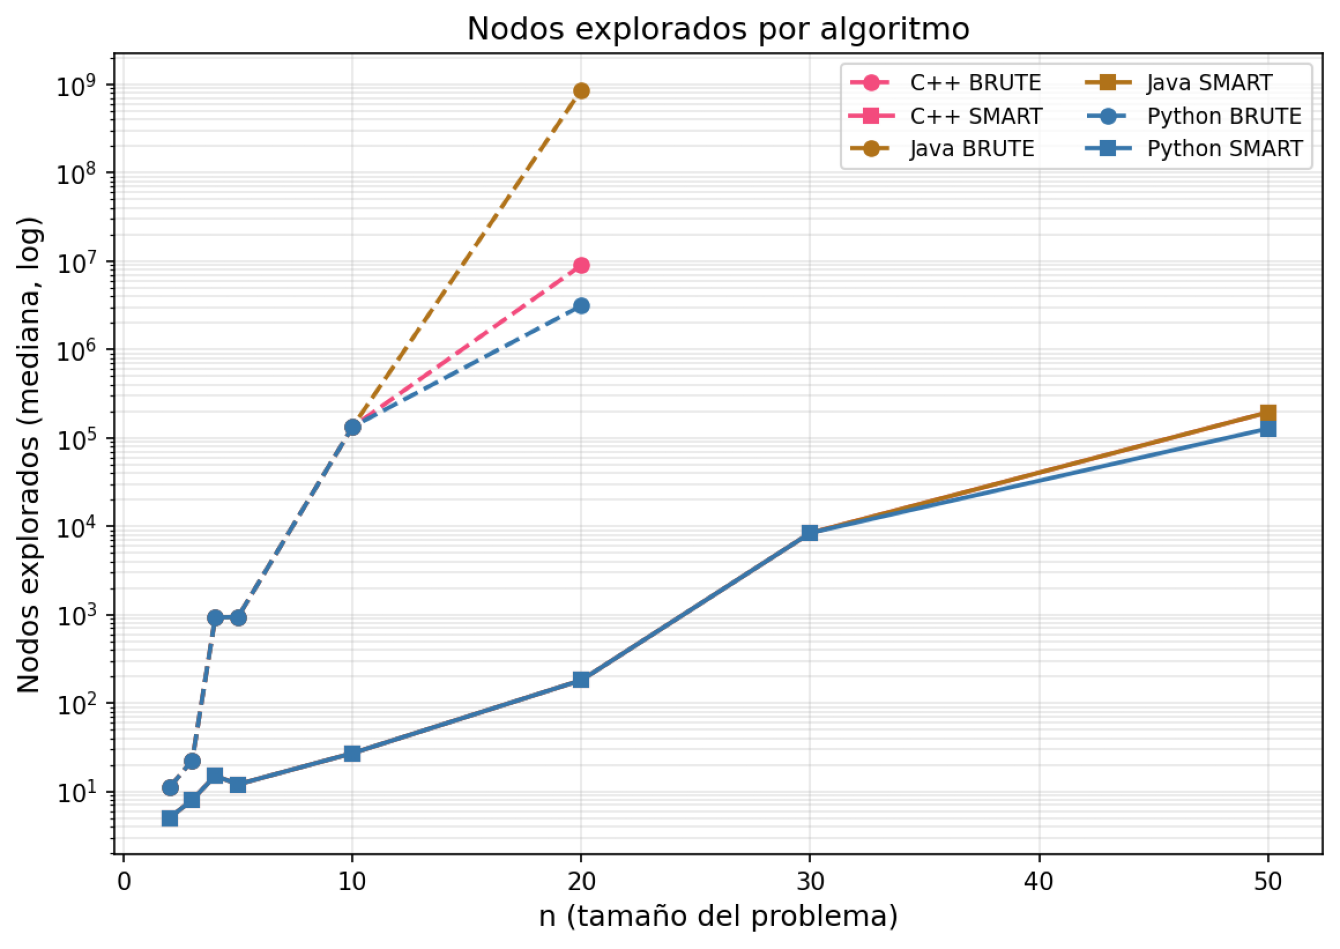
\includegraphics[width=0.85\textwidth]{figuras/nodes_explored.pdf}
\caption{Nodos explorados por algoritmo en función de $n$ (escala logarítmica).}
\label{fig:nodes}
\end{figure}

\subsection{Timeouts y casos difíciles}
\label{sec:exp:timeouts}

\begin{figure}[htbp]
\centering
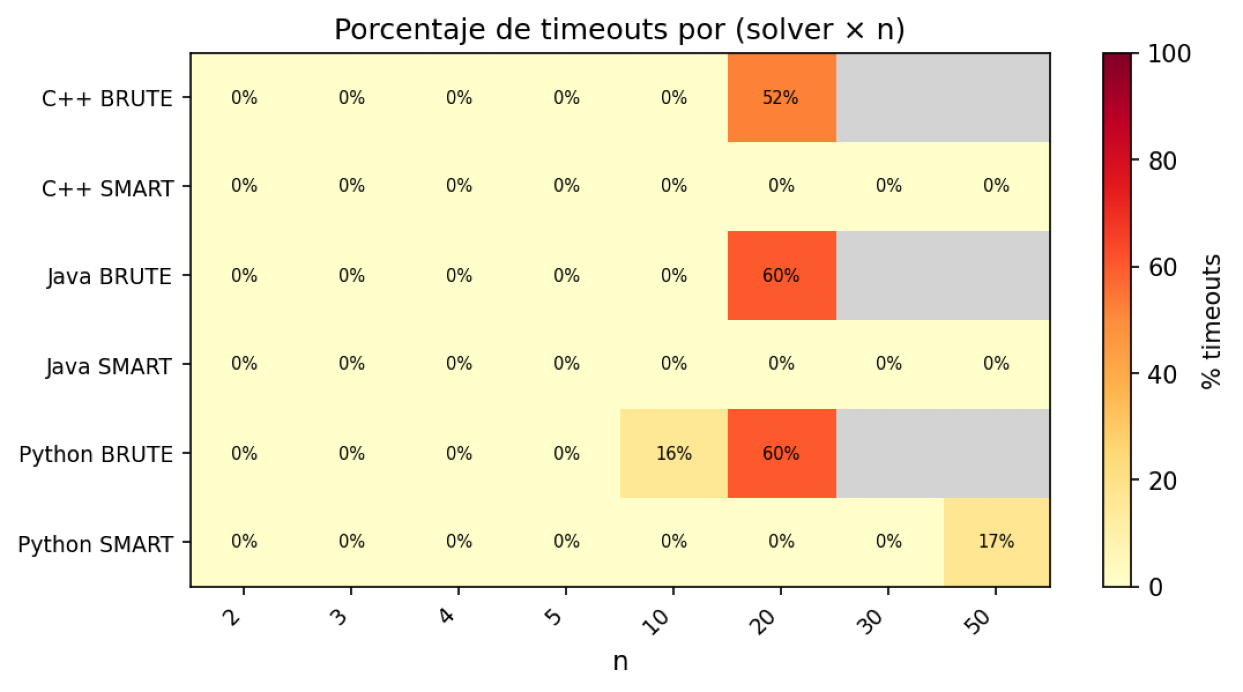
\includegraphics[width=0.95\textwidth]{figuras/timeouts_heatmap.pdf}
\caption{Porcentaje de timeouts por (solver $\times$ $n$).
         El gris indica celdas sin datos.}
\label{fig:timeouts}
\end{figure}

La Figura~\ref{fig:timeouts} y la Tabla~\ref{tab:summary_by_n} muestran el
patrón de timeouts.  Los puntos principales son:
\begin{itemize}
  \item BRUTE en Python y C++ comienzan a hacer timeout a partir de $n=20$.
  \item Las instancias de la familia \textbf{hard} (derivadas de fórmulas
        3-SAT cerca del umbral de satisfacibilidad $\rho\approx 4.27$) producen
        timeout en \emph{todos} los solvers desde $n=102$.  Esto muestra el
        peor caso exponencial del problema incluso para SMART.
  \item La instancia $n=100$, $m=200$ no terminó en más de 5~minutos con
        C++~SMART, confirmando la intractabilidad para instancias grandes.
\end{itemize}

\begin{center}
\input{tablas/summary_by_n.tex}
\end{center}

\begin{center}
\input{tablas/summary_by_family.tex}
\end{center}

\subsection{Anomalías y observaciones adicionales}
\label{sec:exp:anomalias}

\begin{enumerate}
  \item \textbf{Warm-up de Java.}  La primera réplica de Java tarda 3--4$\times$
        más que las réplicas siguientes en instancias pequeñas (JIT
        \textit{compilation warm-up}).  Las medianas de tres réplicas mitigan
        este efecto.
  \item \textbf{Variabilidad de Python~BRUTE.}  El tiempo varía
        significativamente entre semillas porque la estructura del árbol de
        búsqueda depende del orden de las tripletas.
  \item \textbf{Instancia patológica.}  Para $n=30$, $m=120$, semilla~s1,
        Python~SMART tardó~24~s frente a $\sim$1~s para otras semillas del
        mismo tamaño; C++ resolvió el mismo árbol en~268~ms.  Esto ilustra
        que el overhead de Python es especialmente costoso en instancias con
        mucho backtracking.
  \item \textbf{Bug C++} \texttt{--time-limit} (documentado en
        Sección~\ref{sec:impl:bug}).
\end{enumerate}
